\begin{figure}[p]
\centering
\begin{tikzpicture}[x=1cm,y=1cm]
\node[anchor=south west,inner sep=0] at (0,0) {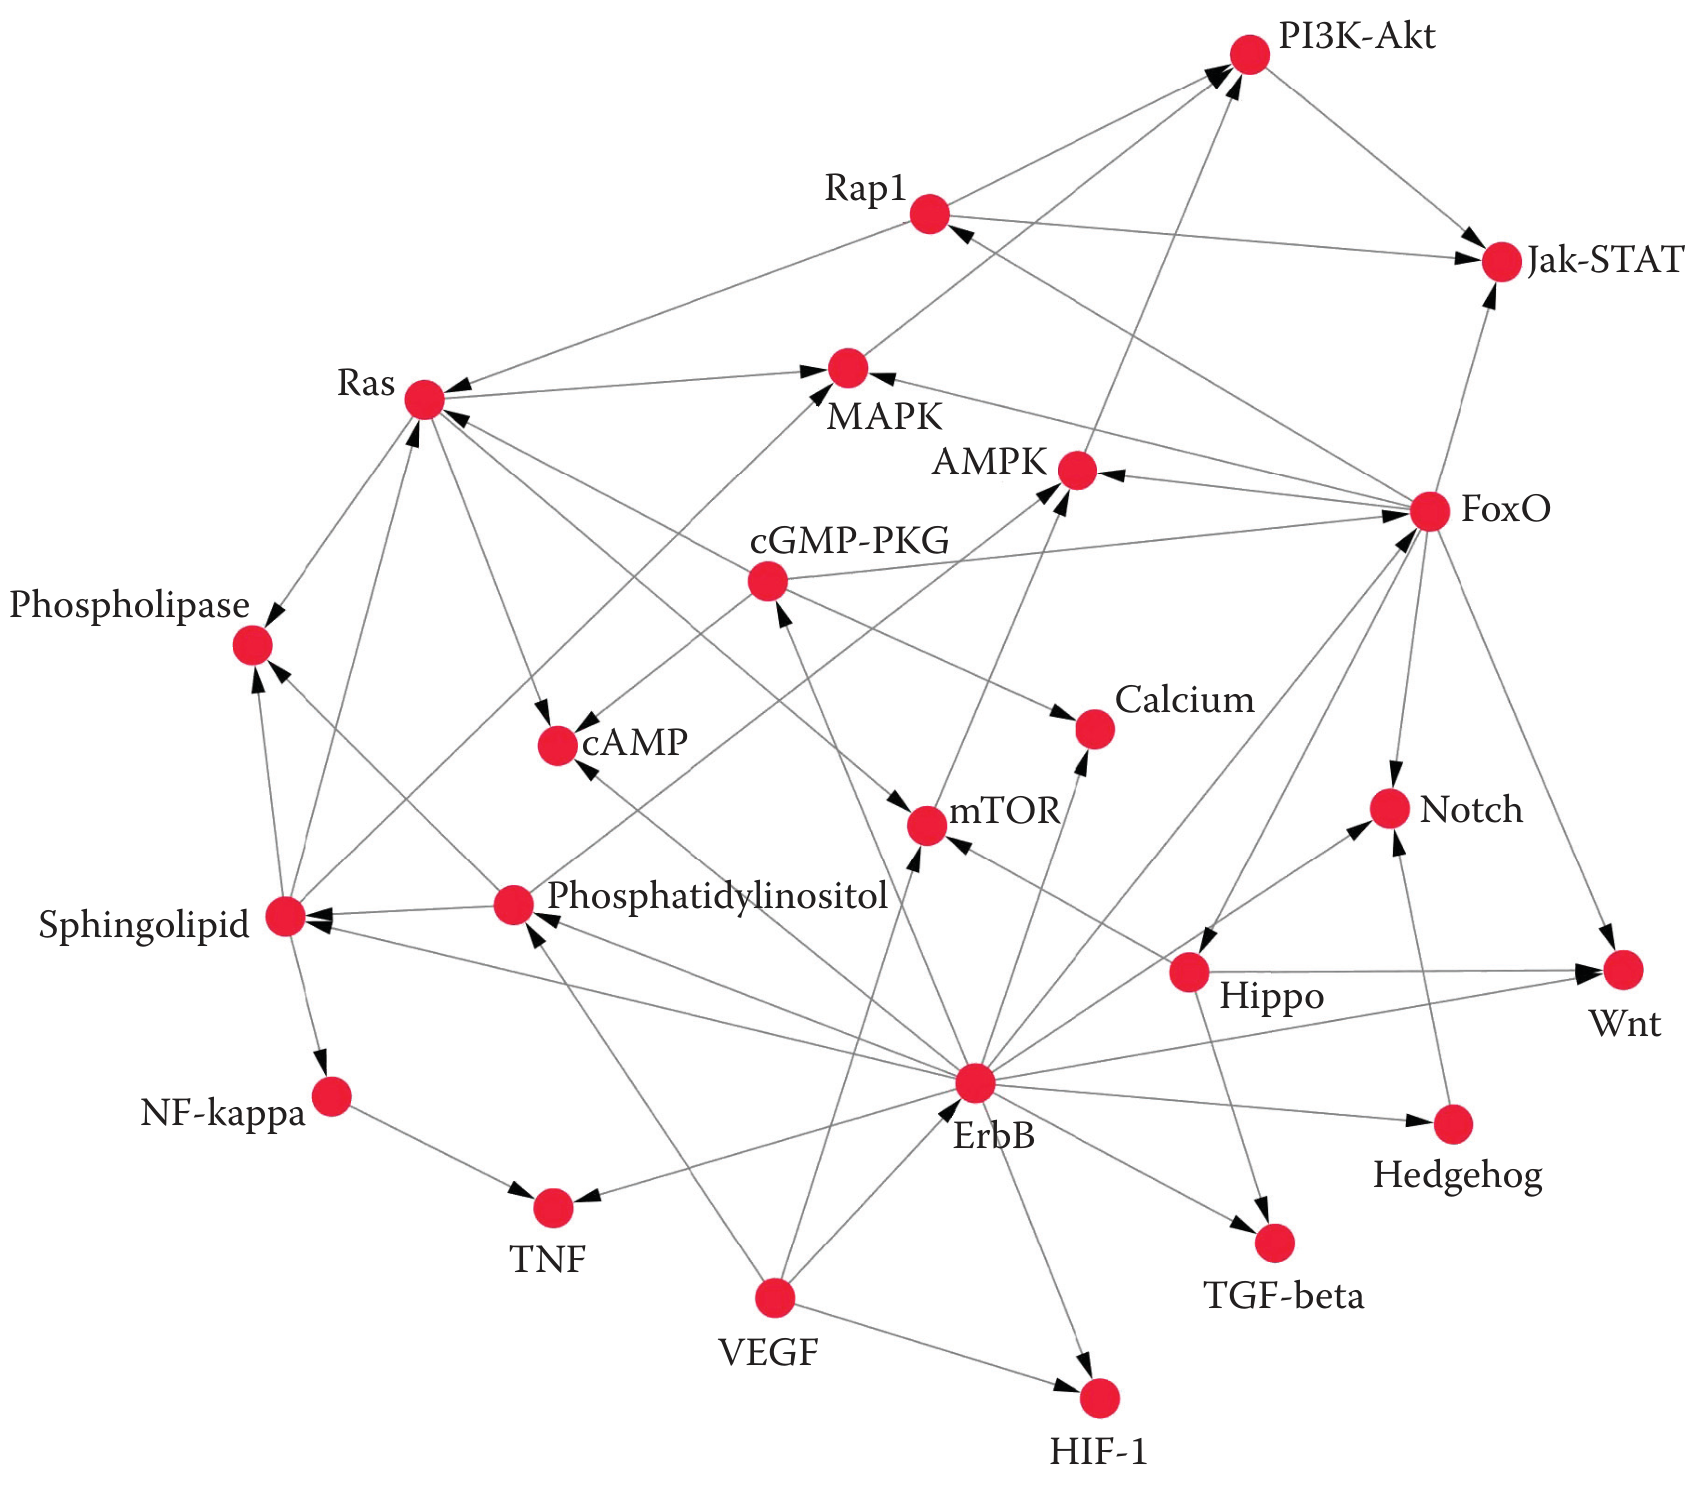
\includegraphics[width=13.5cm]{figures/ch04a_fig22_data.png}};
\fill[white] (0.0438,6.9083) rectangle (2.0215,7.2778);
\node[inner sep=0pt,fill=white,rotate=0,font=\fontsize{8}{8}\selectfont] at (1.0326,7.0930) {磷脂酶};
\fill[white] (0.2795,4.3539) rectangle (2.0232,4.7234);
\node[inner sep=0pt,fill=white,rotate=0,font=\fontsize{8}{8}\selectfont] at (1.1514,4.5387) {鞘脂};
\fill[white] (8.8776,6.1496) rectangle (10.0530,6.5192);
\node[inner sep=0pt,fill=white,rotate=0,font=\fontsize{8}{8}\selectfont] at (9.4653,6.3344) {钙};
\fill[white] (4.3388,4.5856) rectangle (7.1204,4.9551);
\node[inner sep=0pt,fill=white,rotate=0,font=\fontsize{8}{8}\selectfont] at (5.7296,4.7703) {磷脂酰肌醇};
\end{tikzpicture}
\origfig{22}{结合整数规划的低秩表示诱导结构方程模型估计的24条信号转导通路调控网络。}
\label{fig:ch04a-22}
\end{figure}
